
\documentclass[12pt]{article} % use larger type; default would be 10pt

\usepackage[utf8]{inputenc} % set input encoding (not needed with XeLaTeX)

%%% PAGE DIMENSIONS
\usepackage{geometry} % to change the page dimensions
\geometry{a4paper} % or letterpaper (US) or a5paper or....
\geometry{margin=1in} % for example, change the margins to 2 inches all round
% \geometry{landscape} % set up the page for landscape
%   read geometry.pdf for detailed page layout information

\usepackage{graphicx} % support the \includegraphics command and options

% \usepackage[parfill]{parskip} % Activate to begin paragraphs with an empty line rather than an indent

%%% PACKAGES
\usepackage{booktabs} % for much better looking tables
\usepackage{array} % for better arrays (eg matrices) in maths
\usepackage{paralist} % very flexible & customisable lists (eg. enumerate/itemize, etc.)
\usepackage{verbatim} % adds environment for commenting out blocks of text & for better verbatim
\usepackage{subfig} % make it possible to include more than one captioned figure/table in a single float
% These packages are all incorporated in the memoir class to one degree or another...

%%% HEADERS & FOOTERS
\usepackage{fancyhdr} % This should be set AFTER setting up the page geometry
\pagestyle{fancy} % options: empty , plain , fancy
\renewcommand{\headrulewidth}{0pt} % customise the layout...
\lhead{CS 5150 Milestone 3 Report}\chead{}\rhead{Sun in the City Group}
\lfoot{}\cfoot{\thepage}\rfoot{}

%%% SECTION TITLE APPEARANCE
\usepackage{sectsty}
\allsectionsfont{\sffamily\mdseries\upshape} % (See the fntguide.pdf for font help)
% (This matches ConTeXt defaults)

%%% ToC (table of contents) APPEARANCE
\usepackage[nottoc,notlof,notlot]{tocbibind} % Put the bibliography in the ToC
\usepackage[titles,subfigure]{tocloft} % Alter the style of the Table of Contents
\renewcommand{\cftsecfont}{\rmfamily\mdseries\upshape}
\renewcommand{\cftsecpagefont}{\rmfamily\mdseries\upshape} % No bold!

%%% END Article customizations

%%% The "real" document content comes below...

\title{CS 5150 Milestone 3 Report \\ Sun in the City Group}
\author{Phillip Tischler (pmt43), Brian Toth (bdt25), Vera Khovanskaya (vdk9), \\ 
Sean Salmon (ss2669), Lin Xue (lx39), Zach Porges (zip2),  \\
and James McGuinness (jrm369)}
%\date{} % Activate to display a given date or no date (if empty),
         % otherwise the current date is printed 

\begin{document}
\maketitle
\clearpage
\tableofcontents

%%%%%%%%%%%%%%%%%%%%%%%%%%%%%%%%%%%%%%%%%%%%%%%%%%%%%%%%%%%%%%%%%%%%%%%%%%%%%%%%
\section{Project Description}

The goal of the project is to create a new website and Content Management System (CMS) for the Cornell Daily Sun in a new market: Cornell’s new Tech Campus in New York City. According to the client, Joseph Staehle, IT Manager for the Daily Sun, it should be a ``Totally online, totally tech based newspaper for the tech campus.”

The website is being built using Drupal, but will involve a custom front-end design as well as intelligent back-end technology. The website will include data fusion, aggregation of articles from other news sources.

%%%%%%%%%%%%%%%%%%%%%%%%%%%%%%%%%%%%%%%%%%%%
\subsection{Scope \& Requirements}

The project analyzed in this document is one to build a new website and Content Management System (CMS) for The Cornell Daily Sun. This website will represent a new market for the client. That is, the client is attempting to expand its newspaper to begin bringing news to the students of Cornell University’s new Tech Campus in New York City.
                   
\subsubsection{System Status}
                   
The Cornell Daily Sun website is an existing product that is managed with a Drupal CMS and custom extensions. This project is to build a new website for the Cornell Tech Campus, and is therefore a new product and not an augmentation or replacement. However, if this new website is extremely successful the old website may be converted to the new one. To maintain familiarity with the CMS system, the client has requested the CMS be based on the Drupal CMS.
                   
\subsubsection{Functionality}
                   
There are four required pieces of functionality the project must support: a website for readers to browse the newspaper, a CMS to manage the website and allow writers to post content, a means to allow Data Fusion to present external content inline with content generated by The Cornell Daily Sun, and finally a Brand to associate with this new website. Like the existing CMS The Cornell Daily Sun uses, the CMS must allow the writers and editors to upload their content like articles, blogs, comments, images, and advertisements. The website itself must display this content in a reasonable and convenient way that allows readers to browse and obtain the information they are looking for. To create a unique Cornell Tech campus newspaper, the project also requires the team to create a Brand. This includes a logo, a display name, and a look and feel for this newspaper. A key aspect of this Brand will be Data Fusion, a distinction from the current website the client operates. Data Fusion will present articles from external sources inline with an article posted by the Cornell Daily Sun. It is similar to a ``Read More" link, except this information will be external and automatically presented with the article from The Cornell Daily Sun.
                   
There are three desired but not required pieces of functionality for the project: an optimized mobile version of the site, an algorithm to perform the Data Fusion automatically, and a performance optimizer for the entire system. The mobile optimized site will allow readers to browse The Cornell Daily Sun’s website on a mobile device in a much faster and convenient way than to load the main page onto a slower device with less screen display area. This functionality may require too much time to implement, which is why it is not a required portion of this project. The Data Fusion described in the paragraph above was a framework to allow custom algorithms to link external content as well as manually link content. The other piece of functionality that is not required is an algorithm to automatically detect and link external content to the content generated by The Cornell Daily Sun. This may involve web and RSS feed scraping as well as Machine Learning and other advanced topics. Due to the complexity of the functionality relative to the timeframe of the project, this functionality has been deemed not required. However, if implemented it will save time, make running the website easier, and increase the attractiveness to potential readers as it will dynamically update the site. The final desired but optional piece of functionality is a performance optimization that will decrease the time it takes to load the website. Using a 50Mbps connection (an average user only has access to a 2Mbps connection), the client’s current site takes over 5 seconds to load the visible page of the homepage and over 13 seconds to load the entire page. Most websites can respond in under 200 milliseconds and load completely in a second. Every millisecond the user waits has a psychological impact on their perception of the website, and thus it is critical to load as fast as possible. There are simple upgrades to the system that can be employed to achieve this goal. However, time and budget may be a limiting factor, which is why this functionality is desired but not required.

\subsubsection{Dependencies}
                   
Drupal. Drupal is an open-source CMS that The Cornell Daily Sun uses for their current website, and as such the CMS that will be used for this project. The Drupal CMS is licensed under the GNU General Public License. This license is explained under the discussion of business considerations. Drupal is composed PHP, HTML, and CSS to generate and display the content, and a MySQL database to store the information composing the content itself. Drupal 6 requires PHP 4.4.0 or higher, while Drupal 7, the latest release, will be used and it requires PHP 5.2.5. Drupal provides a large baseline of features for a website, including but not limited to, user account handling, layout management, website menu customization, RSS feed aggregation, article search, and FTP access. Extensions can be written for Drupal in PHP, and there are over 17,000 free extensions available that are also under the GNU General Public License. For this project, Drupal will provide a very strong base for building this system.
Deployment Server. We will be using a Linux-based server hosted on a cloud platform for purposes of development and eventually deployment. The plan is to use Amazon AWS as the cloud provider. Because Drupal uses PHP and MySQL only, a Linux server is appropriate.
Data Fusion. The Data Fusion extension will most likely be integrated into Drupal using a PHP module, but the core functionality of the scraper will be written in Java. Because Drupal already has RSS aggregation, it is very likely that the module will rely on some form of RSS news scraping to find similar news articles.
Apache Lucene. The Data Fusion algorithm will be using the Apache Lucene indexing and search library that is licensed under the Apache 2.0 license. This license has been vetted and determined appropriate for this project.
                    

%%%%%%%%%%%%%%%%%%%%%%%%%%%%%%%%%%%%%%%%%%%%
\subsection{Benefits}

There are two unique stakeholder entities that will benefit this project. The first is The Cornell Daily Sun that will own the product that results from the project. The second is the students and other community members of Cornell University’s new Tech Campus. Each entity will benefit in different ways from the success of this project.
                   
\subsubsection{Cornell Daily Sun}
                   
With the new website, The Cornell Daily Sun will both expand its market, increase its influence, and increase its revenue. This project will allow the client to new types of content for both its paper based and web based publications. As the website matures, the project will allow the client to attract new readers on the order of 80,000. As the website displays advertisements, there will be a new source of income for the Cornell Daily Sun. Finally, with the new content and new readers in the New York City area, the website is very likely to attract new advertisers.
                   
Another potential benefit of the project is the integration of new technology. That is, the current website the client runs is on an older Drupal 6 CMS whereas the new website will be built with Drupal 7. Our new design will better organize the website content, and eciency code will be used to improve the compiling time from minutes to seconds. The Drupal 7 has major improvements over the Drupal 6. They are enhanced security (for scheduled tasks, password, and log-in), usability (better support for both administrators and users), and performance (new features for search, file handling, and RSS feeds). These new technical improvements are desired in the current Cornell Daily Sun website. If this project is a success, it can be deployed to replace the current website as well.
                   
\subsubsection{The Cornell Tech Campus Community}
                   
The website to be developed provides a way for broadcasting current news about the Cornell NYC Tech campus, which serves the Tech campus members and the general Cornell community. With blog services in addition to news, the website also enables individuals to share information with the community about tech topics, their life, campus life, alumni activity, and career experience. 

%%%%%%%%%%%%%%%%%%%%%%%%%%%%%%%%%%%%%%%%%%%%%%%%%%%%%%%%%%%%%%%%%%%%%%%%%%%%%%%%
\section{System Design}

The system has been designed to be as modular and uncoupled as possible. The Cornell Daily Sun’s current website is highly coupled and has prevented them from upgrading their system form Drupal 6 to Drupal 7.

The website will be hosted on Amazon AWS running an Apache 2 Web Server and a MySQL Database Server. Drupal 7 will be used to provided the base CMS and website structure. The team will develop custom XHTML, CSS, and PHP to create a ``theme" in Drupal. This customization can easily be ported to other Drupal versions and is a lightweight display layer. This will generate the viewable site and handle HTTP requests.

\begin{figure}[htbp]
\begin{center}
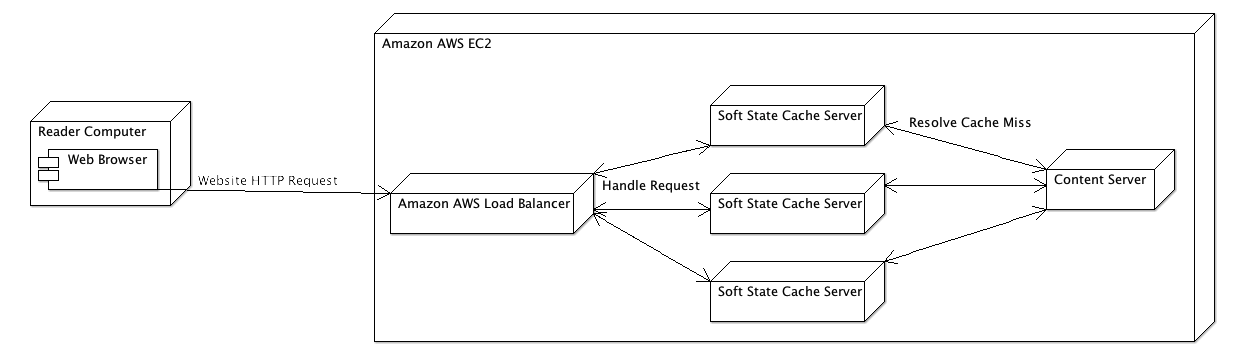
\includegraphics[width=6in]{images/data_flow}
\caption{Deployment Diagram}
\end{center}
\end{figure}

A Varnish server will be used as a soft-state in memory cache server. It works as a reverse proxy HTTP server and can handle about 3,000 page requests a second. This will provide incredible performance and scalability of the new site. Drupal also has pre existing modules to integrate with Varnish. This allows Drupal to invalidate page cache entries as the website is updated by The Cornell Daily Sun and happens completely behind the scenes.

Java will be used for the Data Fusion algorithm. The first component is RSS and Website Feed scraping. Various libraries are being analyzed to handle this workload. Essentially, the program will listen to RSS feeds and store the data in a MySQL database. Another component, the indexer, will take the data that has been scraped and put it into an Apache Lucene Index. Finally another component, the data fusion algorithm, will use the meta-tag taxonomy of an article to search for relevant data in the RSS and Website Apache Lucene Index, and store likely matches in another MySQL table.

To choose which Data Fusion articles get posted on the website, the team will build a lightweight PHP Drupal Extension to allow editors to approve fusion results as well as add in manual fusion data. This module will be an extremely lightweight and as decoupled as possible.

\begin{figure}[htbp]
\begin{center}
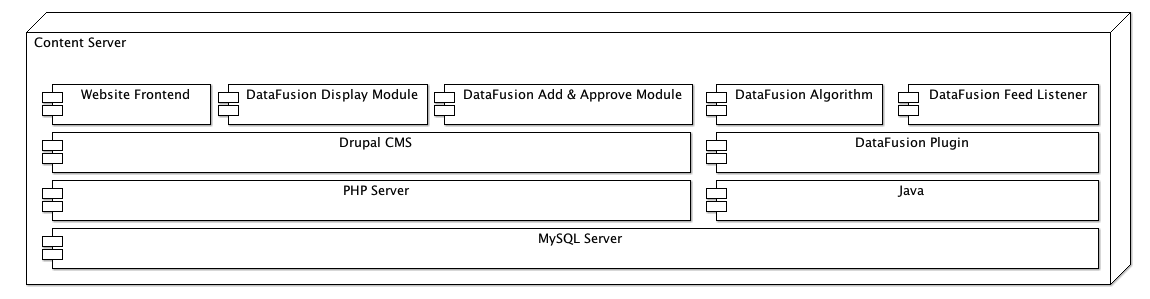
\includegraphics[width=6in]{images/software_stack}
\caption{System Architecture}
\end{center}
\end{figure}


%%%%%%%%%%%%%%%%%%%%%%%%%%%%%%%%%%%%%%%%%%%%%%%%%%%%%%%%%%%%%%%%%%%%%%%%%%%%%%%%
\section{Milestone Progress}

For Milestone 3 the team finished development of the core system. The website in its current state is sufficient enough to be deployed and client facing. Our team has also completed an initial version of the optional systems like the RSS / Website scraper and data fusion backend. The remaining portion of the project includes: finishing touches on optional components, rigorous code and user testing, integration of news sources and ad sources, and deployment to a production server.

%%%%%%%%%%%%%%%%%%%%%%%%%%%%%%%%%%%%%%%%%%%%
\subsection{Cornell Daily Tech Brand}

In order for the website to be successful once deployed it must convey an exceptional brand. In Milestone 2, our team determined what identity the website should have. For this milestone, we determined what the Cornell Daily Tech brand is, how it should be represented, and how this impacts the website. After many discussions with the Cornell Daily Sun, the team settled on a design aesthetic that is very similar to the one on the Sun’s main website in order to capitalize on a previously adopted, rigorously designed, and well executed brand.


\subsubsection{Requirements}

The team wanted the website to resemble the existing Cornell Daily Sun, so our branding requirements largely stemmed from incorporating existing design moves. However, some requirements were unique to the tech campus website, such as the creation of the logo, the visual negotiation of temporary vs. permanent navigation, and development of a layout. This layout needs to showcase tech content and be visually cooperative with the initial proposed posting style of the news website.

\subsubsection{Design \& Rationale}

Our logo design was one that visually combined symbolic representations of Cornell with symbolic representations of “the city” (NYC). To that effect, we iterated a logo that would use the Cornell Clock Tower and a city skyline. The initial design and color scheme was greyscale on a white background with a calibrated balance of positive and negative space so it could go onto a darker background.  We then iterated on the design and changed the logo to adapt the existing aesthetic of the Cornell Daily Sun.

\begin{figure}[htbp]
\begin{center}
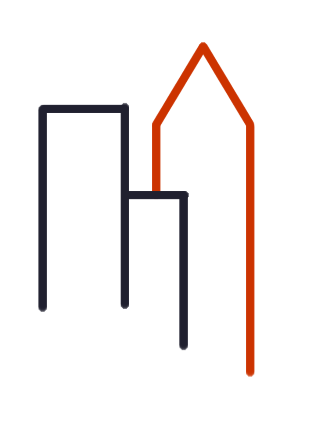
\includegraphics[width=1.5in]{images/logo_old}

\includegraphics[width=1.5in]{images/LogoOnRed_new}
\caption{Logo Old \& New}
\end{center}
\end{figure}

The navigation system was inspired both by NYTBits and the existing cornell website. The idea of having temporary tags or navigation came from NYTBits, so we thought it would be reasonable to have some design moves from their website. However,  we also wanted to keep with the traditional print aesthetic of the Cornell Daily Sun. We accomplished this design with a print line to separate the temporary tags from the permanent ones.

The grid layout was inspired by The Verge, but was also proposed by the client as a reasonable way to present a slowly changing set of articles. The grid layout, in contrast to traditional print layouts, is a good way to recognize the modern aspect of the website without completely disregarding traditional design cues.

\subsubsection{Implementation}

Our implementation method for branding was largely in conjunction with the website interface. We met with the client once to discuss branding verbally and then corresponded over email with mock images of various screens (made in Adobe Fireworks and Adobe Photoshop.) There was iteration based on those conversations and on in-group aesthetic judgements. After some initial coding efforts were made, the design was iterated in HTML as opposed to image representations, with the exception of the logo.

\subsubsection{Results}

We now have an aesthetically reasonable brand for the news website that both follows from the existing Cornell Daily Sun aesthetic, but also recognizes the unique needs of the new website through design innovation in the logo, navigation, and content layout.

%%%%%%%%%%%%%%%%%%%%%%%%%%%%%%%%%%%%%%%%%%%%
\subsection{Website Interface}

For Milestone 2 the team completed an initial base website that was iterated on for Milestone 3. The current website interface is production ready and has passed design requirements and inspection by the client.

The website interface involved modifying Drupal to build a news website custom for the Sun’s content for the Tech Campus.

\subsubsection{Progress}

Modifications since the previous milestone include:

\begin{itemize}
\item Grid layout for articles on the home page
\item Image resizing/formatting
\item Header/background color and spacing
\item Formatting of links in top right corner - trending tags are italicized and separated from permanent tags
\item URLs with tags contain the name of the tag instead of a number (for SEO)
\item Featured article at the top of the home page
\item Improved fonts
\item Formatting of date/time
\item Shadow around content
\item Other minor visual tweaks/enhancements
\end{itemize}

Implementation involved a combination of modifying CSS, installing third-party modules, and modifying Drupal settings. CSS was modified in the sun sub-theme, which overrides CSS from Zen, a simple theme that makes it easy to create sub-themes.

Installed modules include:

\begin{itemize}
\item Nodes in block - used for featured article on home page
\item Menu HTML - used for inserting <em> tags so trending tags can be italicized in menu
\item Pathauto - used for improving URLs for SEO
\item Special menu items - used for the divider between trending tags and permanent tags
\item Views, Views UI - used for the grid of articles on the home page
\item Chaos tools - required for other modules
\item Token - required for other modules
\end{itemize}

\subsubsection{Results}

The front-end of the website, which will be seen by all users, is fairly complete.

\begin{figure}[htbp]
\begin{center}
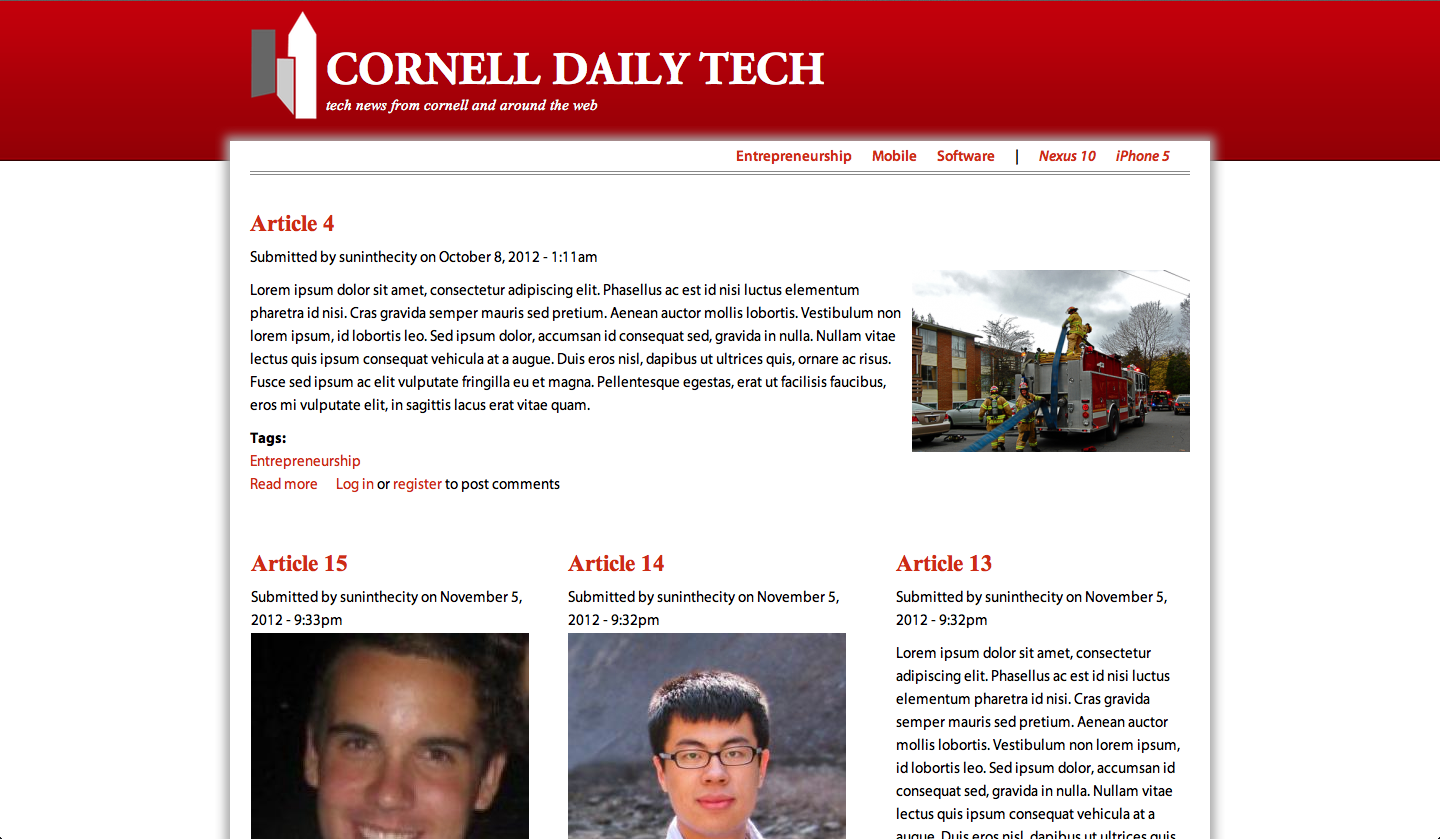
\includegraphics[width=6in]{images/screenshot1}
\caption{The home page. It contains a featured article followed by a grid of 12 articles per page (4 rows of 3)}
\end{center}
\end{figure}

\begin{figure}[htbp]
\begin{center}
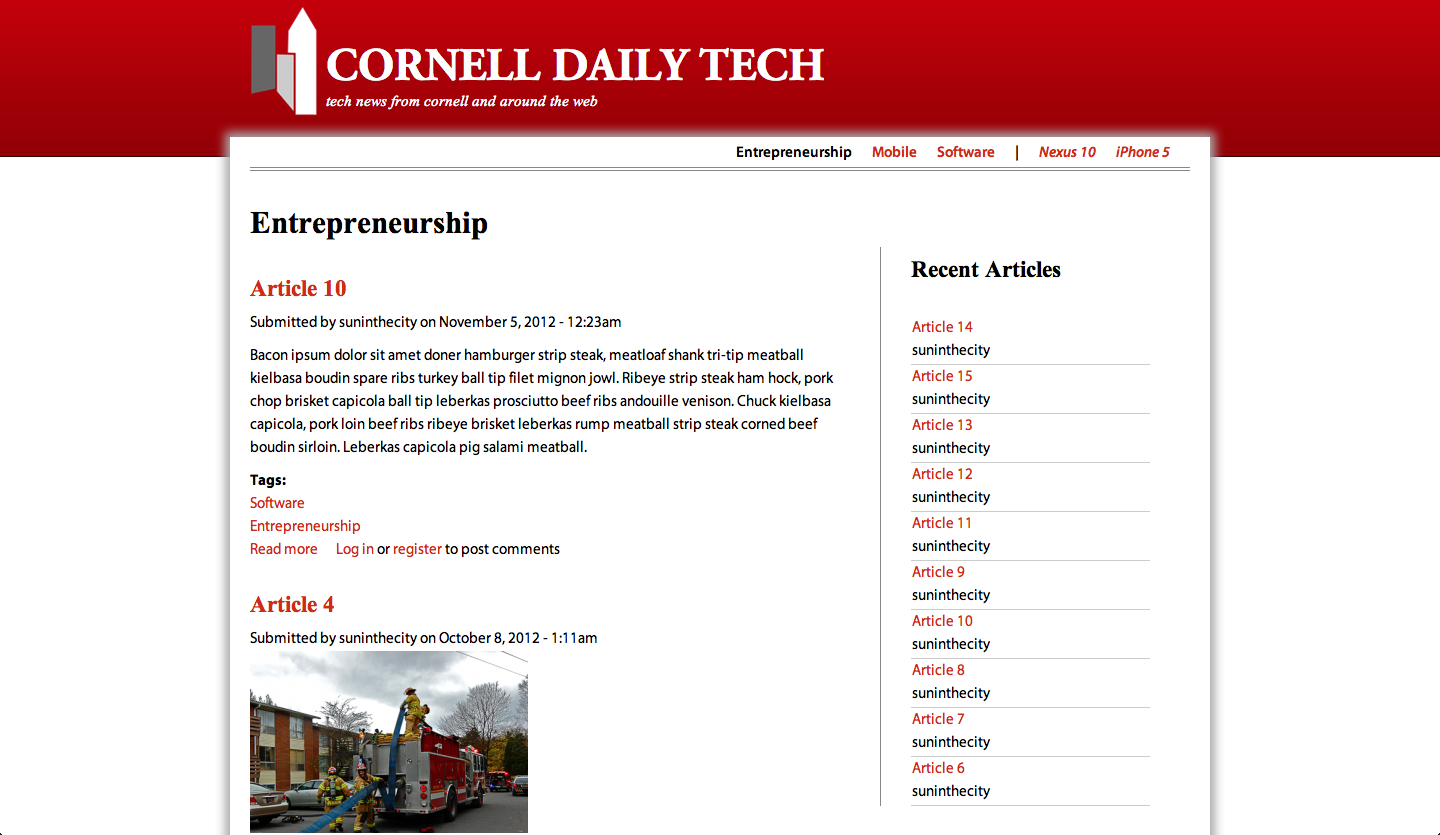
\includegraphics[width=6in]{images/screenshot2}
\caption{All articles that contain a common tag. This view contains just column of articles, with more of a blog style compared with the news style of the home page. The right column contains a list of recent articles, and also contains space for ads.}
\end{center}
\end{figure}

\begin{figure}[htbp]
\begin{center}
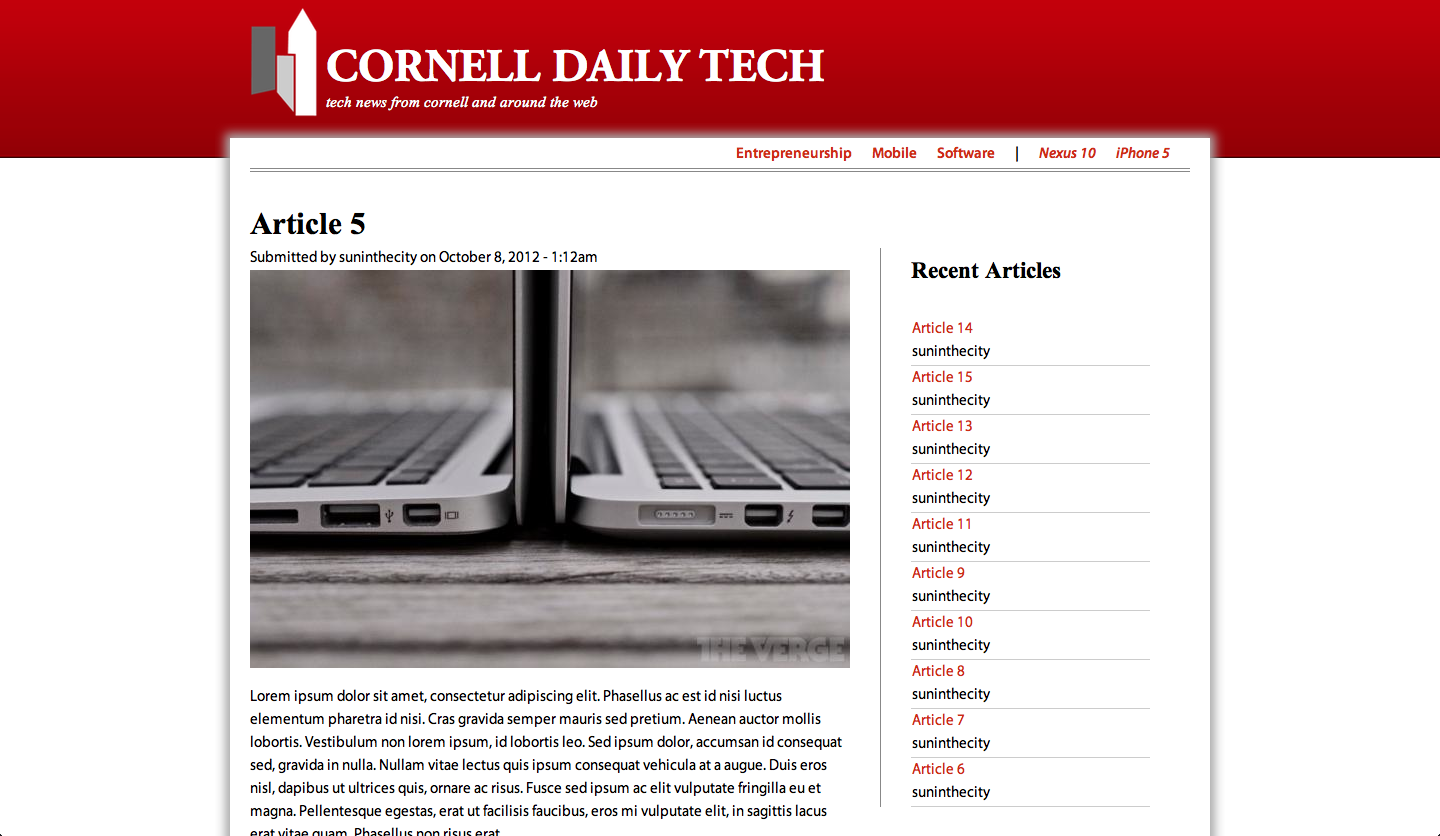
\includegraphics[width=6in]{images/screenshot3}
\caption{A single article with the same two-column layout.}
\end{center}
\end{figure}

%%%%%%%%%%%%%%%%%%%%%%%%%%%%%%%%%%%%%%%%%%%%
\subsection{Database Redesign \& Shared Library}

For this project it was determined that the MySQL database was the natural integration layer for the various components that are developed. For milestone 2 the team developed a database design, and for this milestone we iterated on that design to make it simpler, higher performing, and more complete. The team also created a shared library project to move all common and redundant code to one place.

\subsubsection{Design}

The database was redesigned to the new schema shown below. In the diagram you can see the DataSource table which represents a source of information like The New York Times. Any source can have multiple DataMeans, which represent the generator of source content like The New York Times RSS Feed. These DataMeans objects then generate content which is represented in DataStored. The Data Fusion algorithm then takes various DataStored objects and creates DataFusion objects representing the logical link between external content and content written by The Cornell Daily Sun. The content by The Cornell Daily Sun is represented by a node, which is the article representation in Drupal.

\begin{figure}[htbp]
\begin{center}
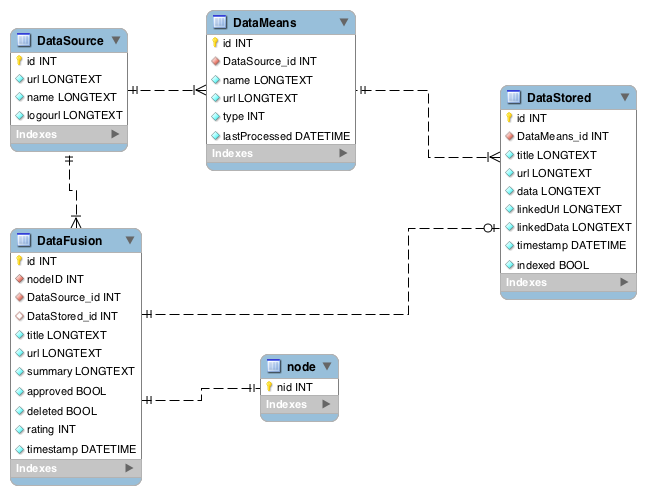
\includegraphics[width=6in]{images/database_schema}
\caption{Database Schema}
\end{center}
\end{figure}

\subsubsection{Implementation Details}

The design was implemented in MySQL WorkBench which allows the design to be changed rapidly and SQL code to be written rapidly. The shared library was written in Java to abstract at a logical level the representation of data. That is, each entry in the MySQL table is modeled as a Java object. The other algorithms interact with the MySQL database through a Manager class that represents the logical operations that would be desired, like get all DataStored objects that need to be indexed. In this way, the logical operations are completely decoupled so that improvements to queries, data storage, and other components can be implemented without affecting the operation of other components.

%%%%%%%%%%%%%%%%%%%%%%%%%%%%%%%%%%%%%%%%%%%%
\subsection{RSS \& Website Scraping}

For Milestone 2 the team developed a design for the RSS \& Website Scraping portion of the Data Fusion process. For this milestone the team coded the scrapers and tested them on various RSS and Website sources. The system can now read external news sources and store them for the data fusion process.

\subsubsection{Requirements}

The RSS Scraping system must retrieve RSS sources in XML format and store them for later use in the data fusion process. The links to HTML sources must then be scraped as these are likely the main article that the RSS feed represents. This will allow the data fusion system to pull RSS sources and website sources together to determine which are appropriate representations of any given article written by the Cornell Daily Sun.

Our team used Java and  put them into another MySQL table. Uses the ROME RSS Parsing Library (which also requires the JDOM XML Parsing Library), as well as a Java to MySQL connector (JConnector) provided free by Oracle.

\subsubsection{Design \& Rationale}

The team decided to use Java as the primary programming language to simplify development, ensure ease of project handover, and ensure the system does not take down the server on which it runs. The team decided to use MySQL as it is the standard web database system to store persistent data, which integrates with Java via JConnector. ROME was used as a library to retrieve RSS and HTML information sources to simplify code development.

\subsubsection{Implementation Details}

The implementation from the previous milestone is the same; names and some functionalities have been changed. The core premise is still retrieving a set of objects (called DataMeans) that contain the necessary information for parsing an RSS feed. This is then passed into ROME and a set of RSS posts are retrieved for that feed. Using a timestamp on the DataMeans object, only the most recent posts are compiled into objects, called DataStored objects, that contain not only the information on the RSS post, but a complete copy of the HTML source the RSS post links to. This data is then written to representative MySQL table.

Changes from previous milestone:

\begin{itemize}
\item No longer is multithreaded. Instead, loops over every RSS feed and then sleeps a set amount of time before iterating over every feed again.
\item Some objects have been renamed for clarity and consistency.
\item Uses a class called Manager for all MySQL query handling and object reading/writing.
\item Uses a DATETIME field in the DataMeans MySQL table for determining whether or not RSS posts should be aggregated.
\item Combined some RSS parsing objects into a single RSS feed parser object (RSSParser).
\end{itemize}

%%%%%%%%%%%%%%%%%%%%%%%%%%%%%%%%%%%%%%%%%%%%
\subsection{Data Fusion Algorithm}

The Data Fusion algorithm has been designed to rely on existing proven systems. The algorithm will take data from various sources and insert them into an Apache Lucene index. Then for each Cornell Daily Sun article it will use the meta-tags (taxonomy) of the article to search the Apache Lucene Index for relevant articles. Finally, it will take the likely matches and insert them into the Data Fusion table.

\subsubsection{Requirements}

The requirements of the data fusion algorithm are to keep track of the data collected by the scraper, search this data with tags provided by article authors, and return relevant relevant results. The system should rank the fusion results and should not repeatedly insert a fused source into a database if it already exists or has been denied by an editor.

\subsubsection{Design \& Rationale}

Apache Lucene is a high-performance, full-featured text search engine written entirely in Java. It is suitable for full-text search, especially cross-platform. Lucene supports parsing query strings with multiple keywords into a Lucene query object and searching with that object. Our requirement of the most matched articles can be fulfilled by utilizing its ranked searching feature -- best results returned first. The direct return from searching the index is the article IDs, which we use to generate DataFusion objects. Therefore, given an article’s tags (taxonomy) the Apache Lucene index that was populated with RSS and Website information can be searched to determine what external sources have similar articles.

\subsubsection{Implementation Details}

The Search method returns an ordered collection of articles ranked by computed scores. The score is calculated for each of the article to match a given query. The scoring model is TfIdf, which can be understood as follows:
\begin{enumerate}
\item Tf: the more frequent a keyword occurs in an article , the greater its score
\item Idf: the greater the occurrence of a keyword in different articles, the lower its score, which means common keywords are less important
\item Multiple keywords: an article that contains more keywords will have a higher score
\item Length normalization: a keyword match in a short article is more important than in a long article
\end{enumerate}

The top 10 matched articles are returned. Each returned article is first found in DataStored by its ID. Then a DataFusion object for it is created. Finally, the result is returned to the MySQL database by calling Manager.createDataFusion.

\subsubsection{Results}

The search module passed the testing with simple inputs within the Java environment. Multiple keywords matching requirement is satisfied. We are doing integrated testing within the data fusion extension with the MySQL database. The testing with the front-end website is expected.

%%%%%%%%%%%%%%%%%%%%%%%%%%%%%%%%%%%%%%%%%%%%
\subsection{Drupal Data Fusion Modules}

The Drupal Data Fusion Modules control the interaction between the Data Fusion system and the website front end by modifying the MySQL database. For milestone 2 the team researched how to customize and extend the core Drupal system. For this milestone the team developed these custom modules which are now ready for the production system.

\subsubsection{Requirements}

The team is required to develop a module that allows writers/editors to add in outside sources relevant to their created articles to be shown alongside with them on the website. Also, this system must allow them to choose which additional information sources populated by the Data Fusion algorithm should be displayed as well.

\subsubsection{Design \& Rationale}

The custom module is designed specifically for ease in accessibility for the writers to navigate through. Once having downloaded the module, each article created on the website has two tabs attached to it titled “Add Source” and “Edit Sources” respectively. These two tabs access to the Data Source, Data Means and Data Fusion tables within the mySQL database.

\begin{figure}[htbp]
\begin{center}
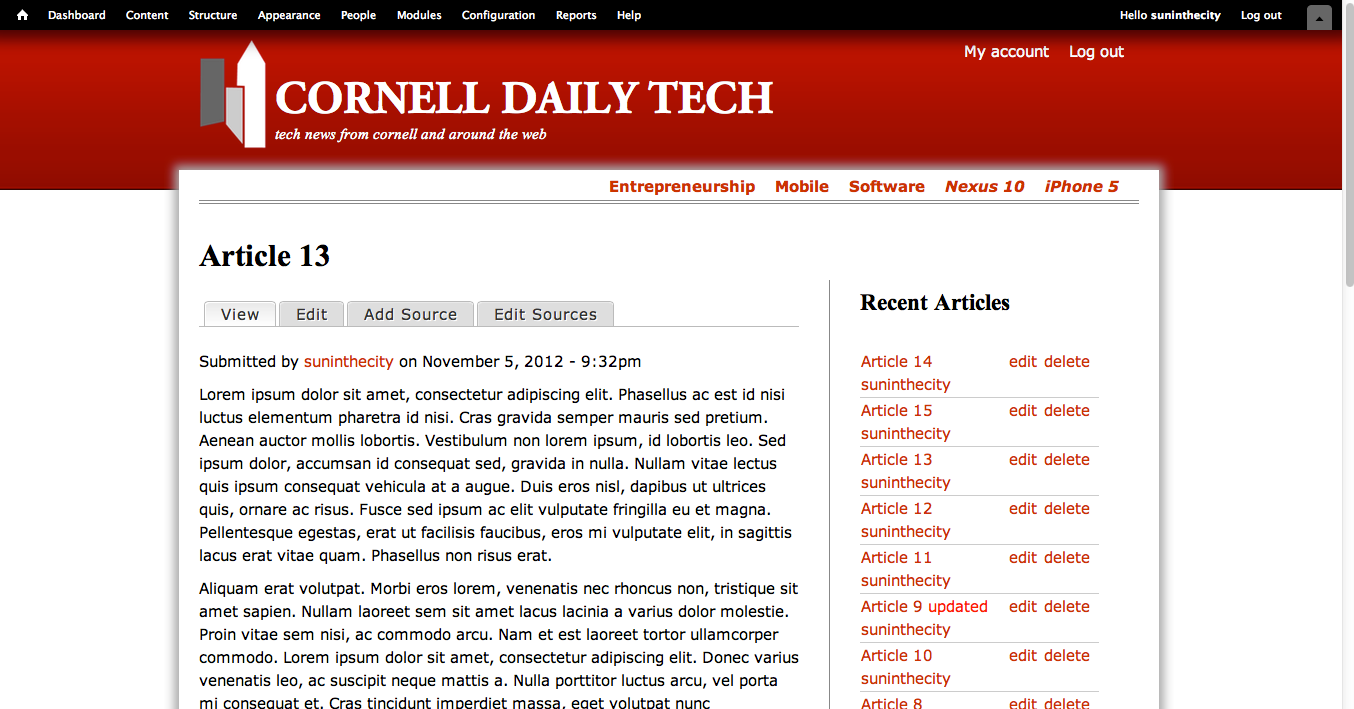
\includegraphics[width=6in]{images/twoTabs}
\caption{The Two Tabs on an Article}
\end{center}
\end{figure}

\begin{figure}[htbp]
\begin{center}
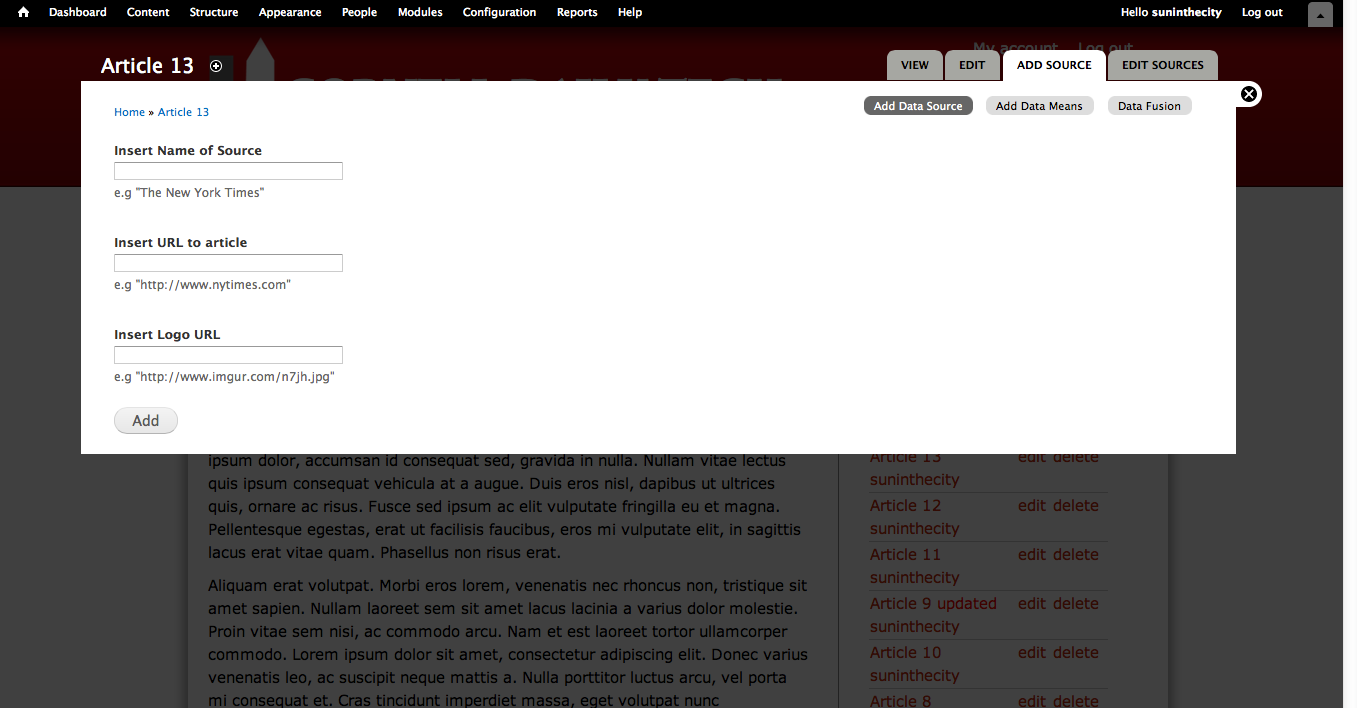
\includegraphics[width=6in]{images/addDataSource}
\caption{Adding a Data Source}
\end{center}
\end{figure}

Under the Add Source tab is an option for the user to enter in an outside Source of data by means of the given fields as shown. Multple text fields allow for writer to clearly see what data needs to be entered where.

\begin{figure}[htbp]
\begin{center}
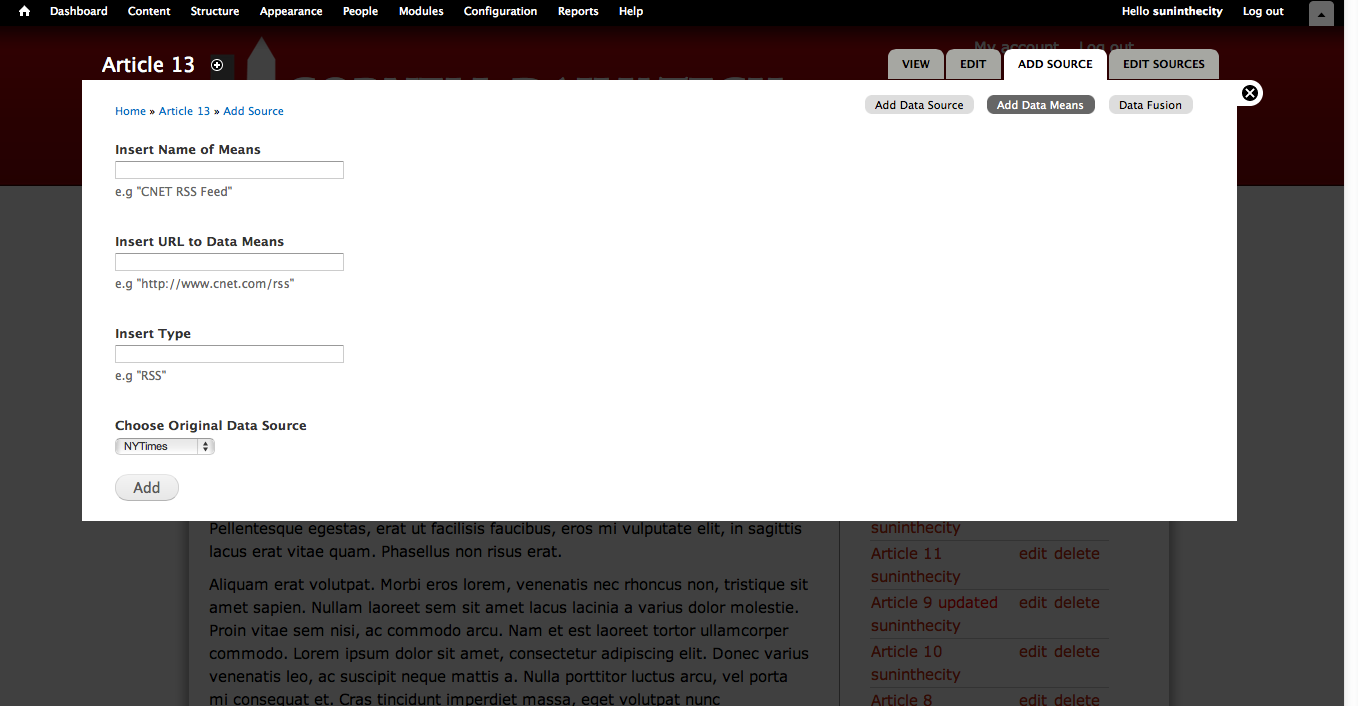
\includegraphics[width=6in]{images/addDataMeans}
\caption{Adding a Data Means}
\end{center}
\end{figure}

After the user inputs these fields and presses add, they can progress to the next page which allows them to optionally add means to their sources with fields for Name, URL and type of source. Since it is infeasible to add a means to a data source without a data source, there is an appropriate selection UI bar which allows the writer to select exactly which data source they would like to add the means to.

\begin{figure}[htbp]
\begin{center}
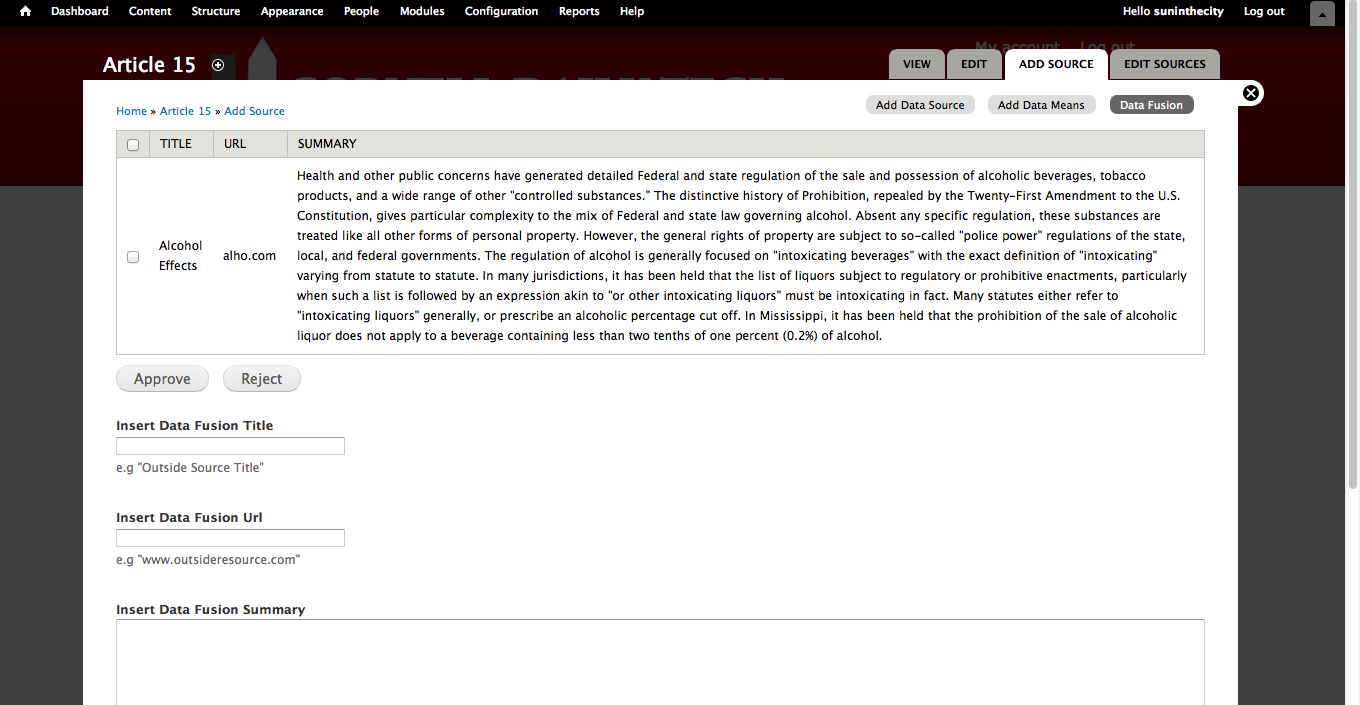
\includegraphics[width=6in]{images/dataFusionTab}
\caption{Data Fusion Tab}
\end{center}
\end{figure}

Lastly, underneath the Add Source branch is a tab for Data Fusion which consists of a table containing every source found by the data fusion scraping algorithm. Within this view controller  are options to approve and reject each data fusion article from being displayed on the website itself as well as options to add in custom Data Fusion elements.

Underneath the Edit Sources tab is the display of all the data sources and data means on the site connected to the selected article. This interface allows the user to clearly select which if any data sources and data means to delete.

\begin{figure}[htbp]
\begin{center}
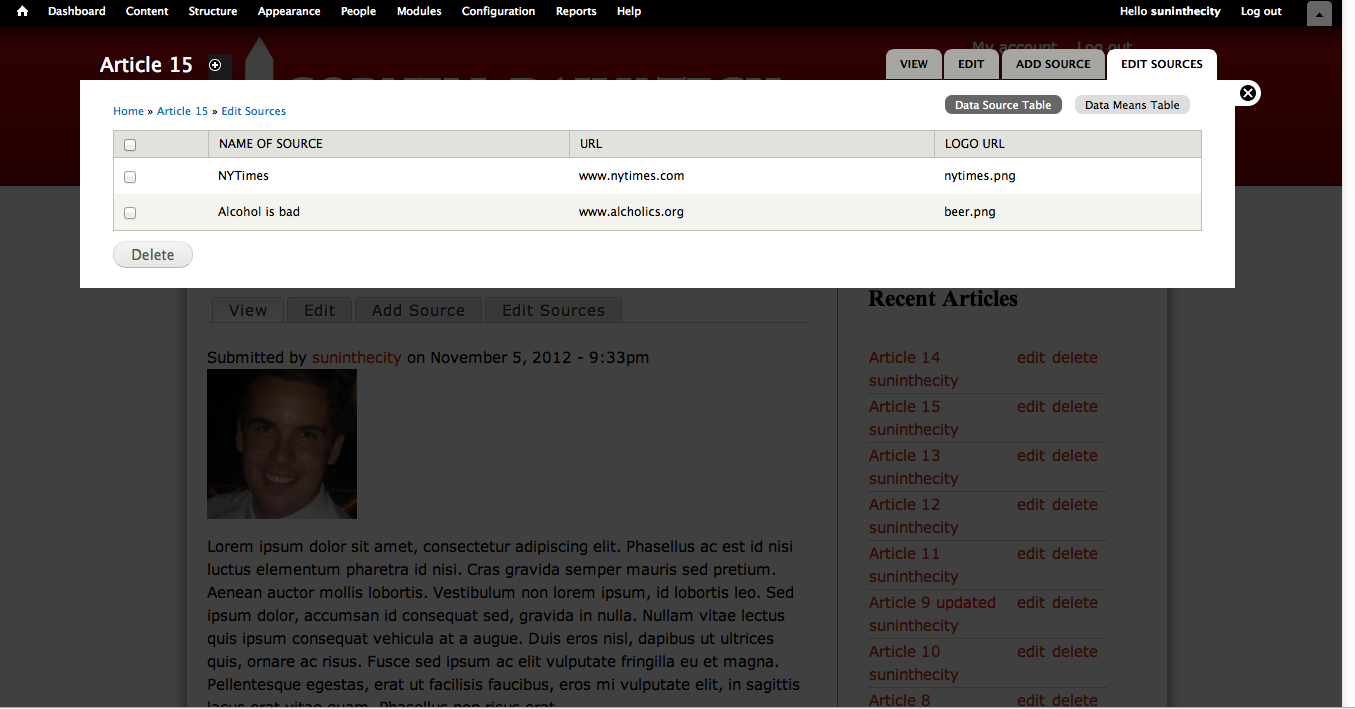
\includegraphics[width=6in]{images/dataSourceTableTab}
\caption{Data Source Table Tab}
\end{center}
\end{figure}

\begin{figure}[htbp]
\begin{center}
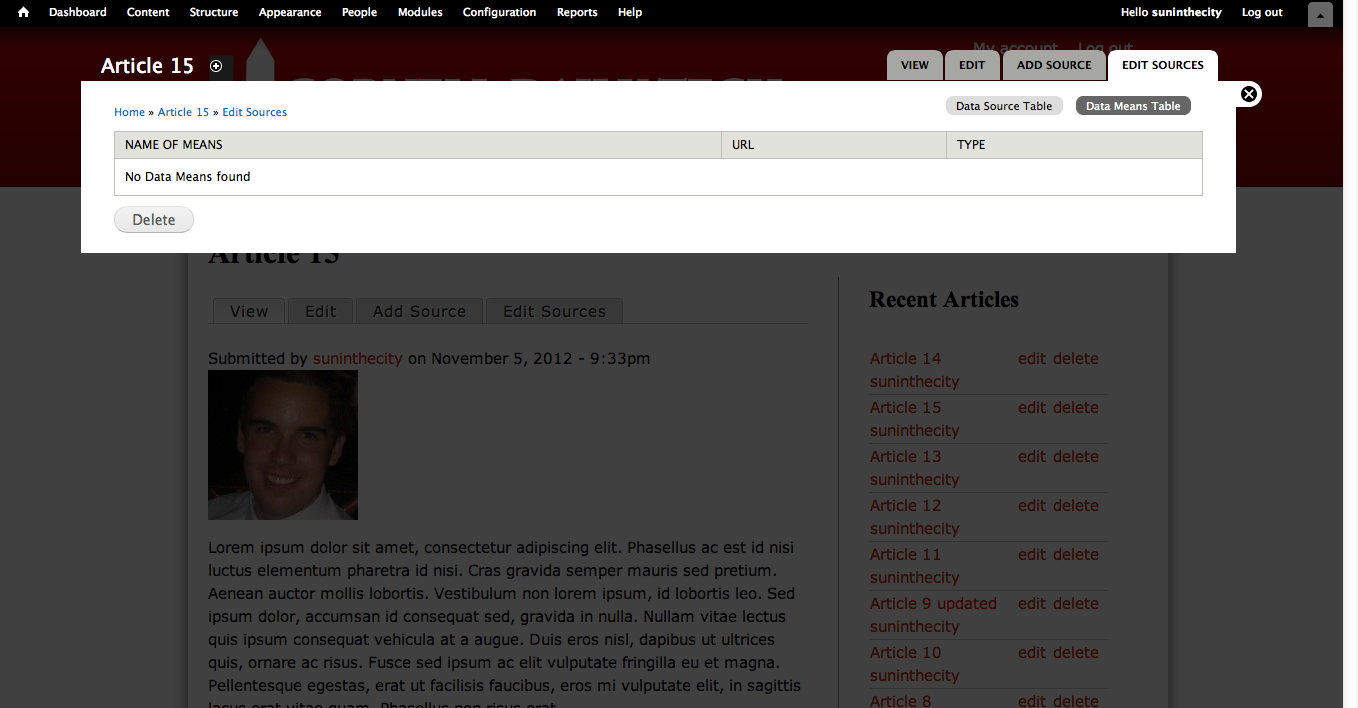
\includegraphics[width=6in]{images/dataMeansTableTab}
\caption{Data Means Table Tab}
\end{center}
\end{figure}

Finally, within the configuration options for the Data Fusion module are the options presented to the editor to ultimately select and approve Data Fusion results for articles and to reject them. Contained in these configurations is the option to remove the Data Fusion Module’s UI on all pages as well as for the editor to add in custom Data Fusion Articles to be displayed alongside the articles.

\begin{figure}[htbp]
\begin{center}
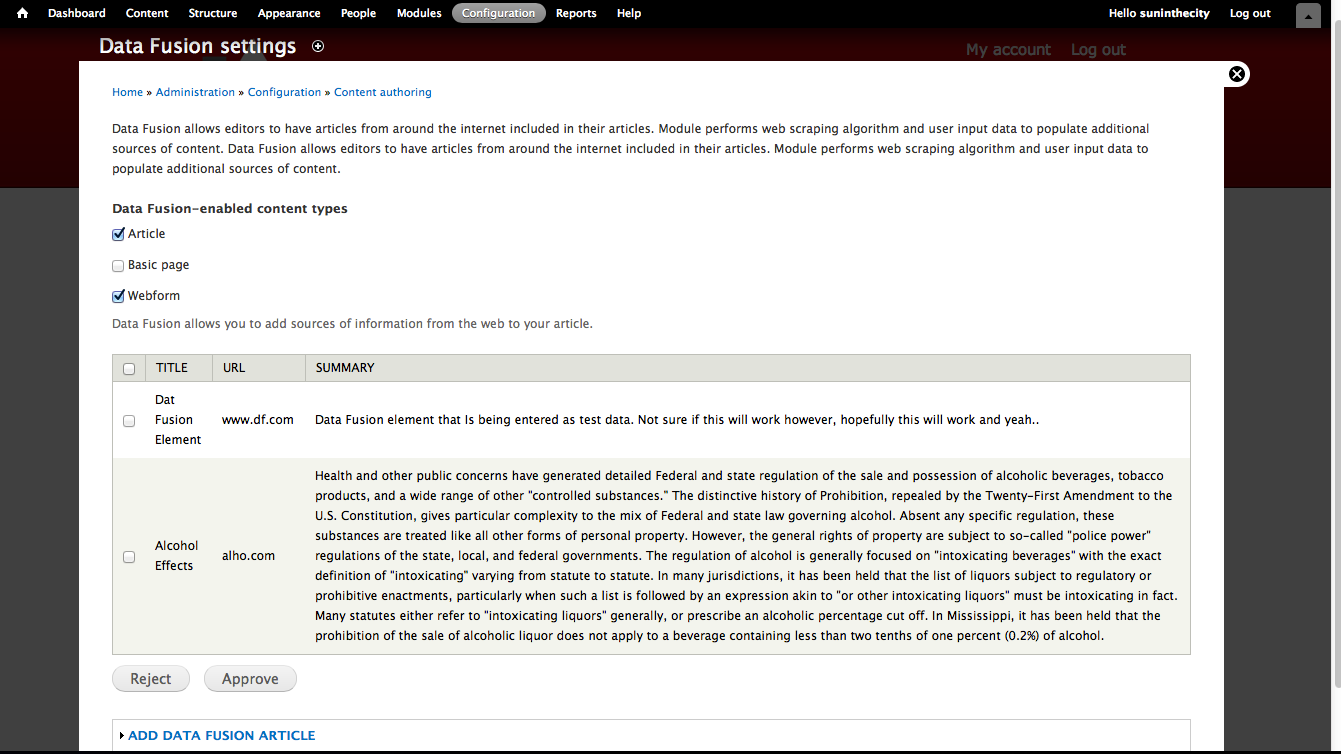
\includegraphics[width=6in]{images/config}
\caption{Configuration}
\end{center}
\end{figure}

\begin{figure}[htbp]
\begin{center}
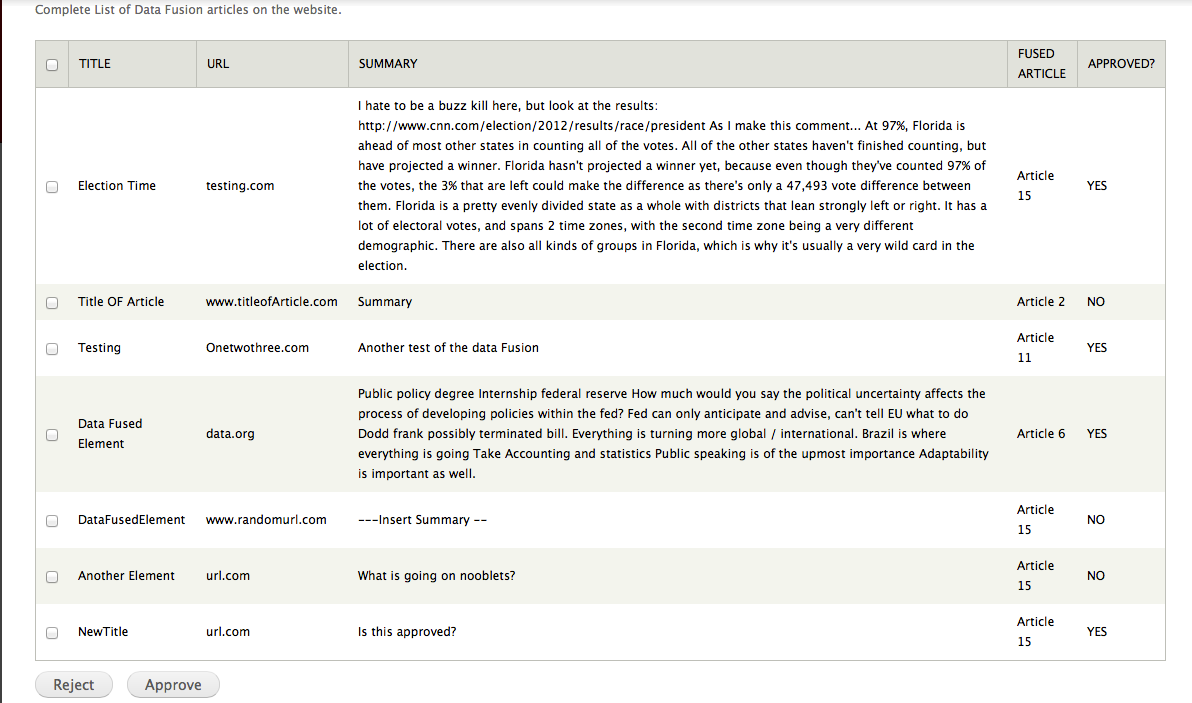
\includegraphics[width=6in]{images/configUI}
\caption{Configuration UI}
\end{center}
\end{figure}

\subsubsection{Implementation Details}

In order to implement this module, it is imperative to have a real-time interaction with the website’s remote mySQL database tables. Through developing php code, HTML, and CSS files it was possible to create the elements displayed within the Module’s UI. Each string of data input by the user is assessed and verified before being entered into the database under their respective tables with appropriate error handling protocols. This module relies on the Data Fusion Algorithm in order to fully function properly.

\subsubsection{Results}

Essentially, this module allows writers to have a simplified and broad access to various sources on the internet pertaining to their article’s content and the ability to include those articles which they deem fitting alongside their article’s display on the website.

%%%%%%%%%%%%%%%%%%%%%%%%%%%%%%%%%%%%%%%%%%%%%%%%%%%%%%%%%%%%%%%%%%%%%%%%%%%%%%%%
\section{Planning}

\subsection{Issues Arisen}

No issues have arisen for this milestone. The next milestone relies on our client’s ability to set up accounts for deployment prior to us needing a server to deploy to. We are in communication with the client to make sure this need is met ahead of our planned development.

\subsection{Schedule}

\begin{itemize}
\item Deadlines
 	\setlength{\itemindent}{2em}
	\item 11/09 - Milestone 4
		 \setlength{\itemindent}{4em}
		\item Brand
		\item Production quality user interface (HTML / CSS)
		\item Data Fusion
		\item RSS Feed obtaining data and storing in database
		\item Algorithm attempting matchmaking
		\item Drupal Modules
		\item Display modules
		\item Data editing modules
 	\setlength{\itemindent}{2em}
	\item 12/07- Milestone 5
		 \setlength{\itemindent}{4em}
		\item AWS Deployment
		\item Integration of Varnish Cache server
		\item Demonstration, Documentation, and Handover
\setlength{\itemindent}{0em}
\item Plan
	\setlength{\itemindent}{2em}
	\item 10/28 - 11/4
		\setlength{\itemindent}{4em}
		\item Finish front end display to user
		\item Finish \& test RSS
		\item Finish \& test Data Fusion Algorithm
		\item Finish \& test Drupal Modules
	\setlength{\itemindent}{2em}
	\item 11/5 - 11/09
		\setlength{\itemindent}{4em}
		\item Milestone 4 presentation
		\item Milestone 4 document
	\setlength{\itemindent}{2em}
	\item 11/09 - Milestone 4
	\item 11/12 - 11/18
		\setlength{\itemindent}{4em}
		\item Final touches to all parts of project
		\item Write example articles
		\item Setup necessary accounts \& google ads
		\item User and system testing
	\setlength{\itemindent}{2em}
	\item 11/19 - 11/25
		\setlength{\itemindent}{4em}
		\item AWS Deployment
		\item Integration of Varnish Server
	\setlength{\itemindent}{2em}
	\item 11/26 - 12/01
		\setlength{\itemindent}{4em}
		\item Validation of requirements and system
		\item Documentation \& Handover
	\setlength{\itemindent}{2em}
	\item 12/02 - Demonstration (Final)
\end{itemize}

Our team has met our internal planned deadlines for this Milestone. The remaining work includes finishing touches, setting up necessary accounts, user and system testing, deployment, validation, and documentation / handover.



%%%%%%%%%%%%%%%%%%%%%%%%%%%%%%%%%%%%%%%%%%%%%%%%%%%%%%%%%%%%%%%%%%%%%%%%%%%%%%%%
\section{Preliminary Documentation}

The following links explain how to setup and build all the separate components of the system. The customized code has been written in JavaDoc format so that a JavaDoc can be generated during the documentation phase of our plan.

\begin{itemize}
\item https://help.ubuntu.com/community/ApacheMySQLPHP
\item http://drupal.org/documentation
\item http://lucene.apache.org/core/4\_0\_0/index.html
\item https://www.varnish-cache.org/docs
\item http://lucene.apache.org/core/
\item http://www.ibm.com/developerworks/opensource/library/os-apache-lucenesearch/
\item http://www.lucenetutorial.com/advanced-topics/scoring.html
\end{itemize}

\end{document}
